\section{Push notifications and power management on iOS}
\label{sec:pushnotification}
\tbd{AL: this section is not intended to be as is in the final report,
but just a collection of results that can be incorporated in the final
document if needed.}

All the following experiments are performed on an \iphone 4 with iOS
6.0.1.  At the beginning of each experiment we close all applications
and restart the \iphone{}. The \iphone{} is connected in \wifi{} to a
controlled access point on which we perform a tcpdump on the \wifi{}
interface and monitor the \wifi{} association between the access point
and the \iphone{}. Each experiment lasts for around 1 hour. 

\begin{figure}
\centering
        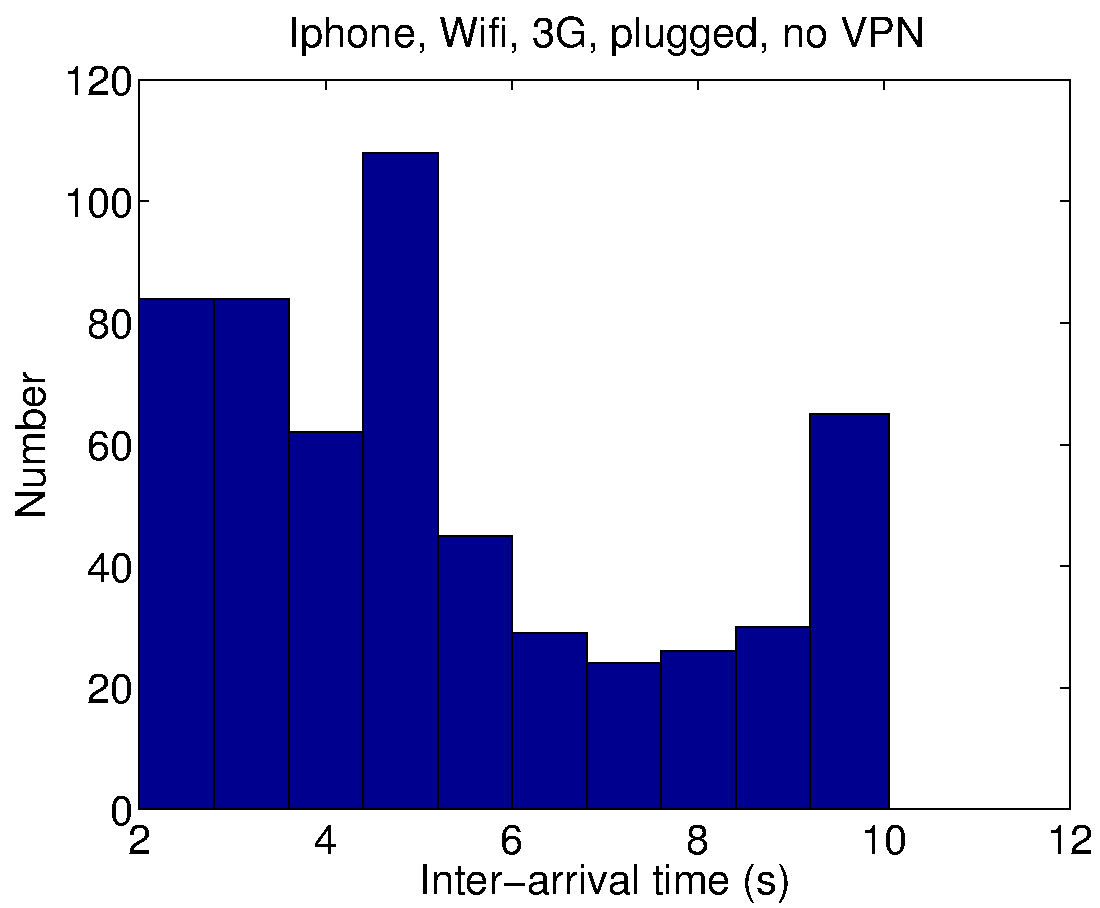
\includegraphics[width=0.8\linewidth]{../../code/pushNotification/Fig/bw_iphone_wifi_3g_plug_novpn_interTs.pdf}
  \caption{Distribution of the interarrival times of Ethernet frames
    for a one hour experiment with an idle \iphone{} plugged-in, with \wifi{} and 3G
    enabled, and no VPN enabled. For each bin of 1 second, we count
    the number of interarrivals in that bin.}
  \label{fig:push_w3p_interTs}
\end{figure}

\begin{figure}
\centering
        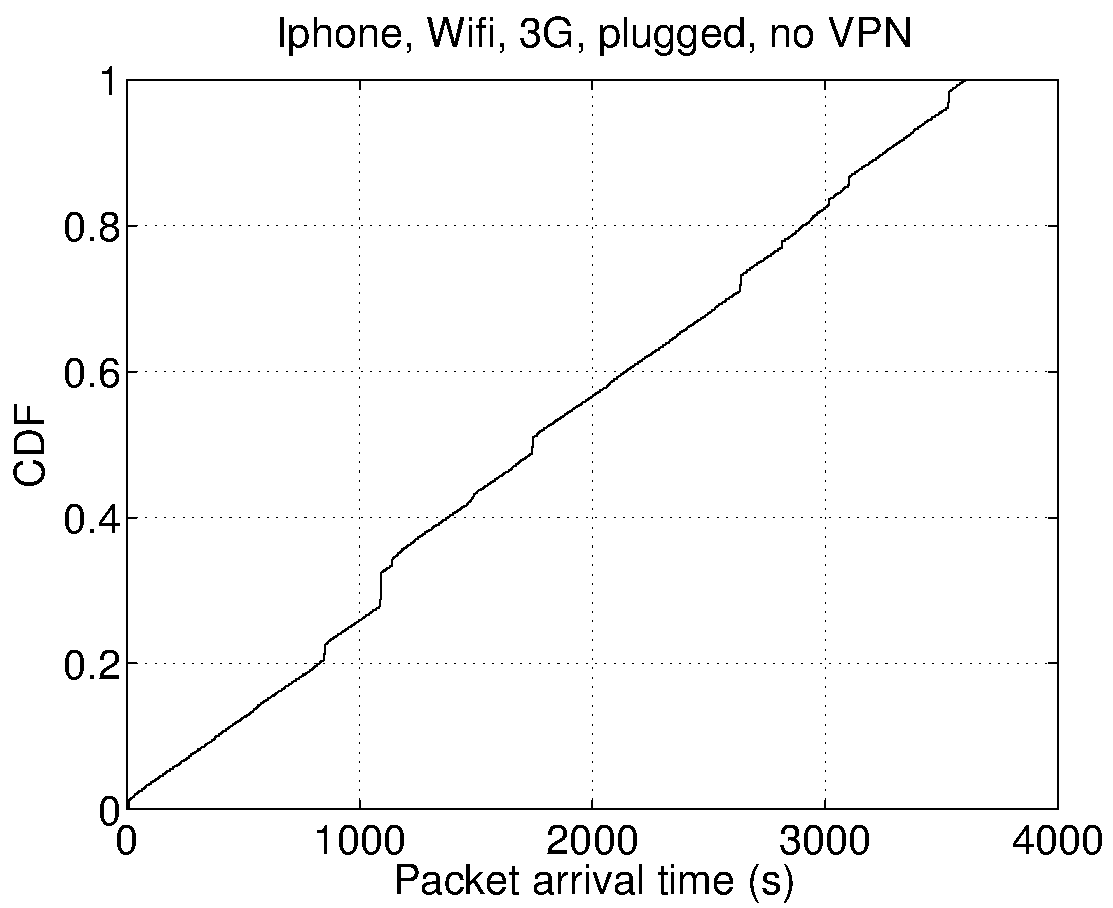
\includegraphics[width=0.8\linewidth]{../../code/pushNotification/Fig/bw_iphone_wifi_3g_plug_novpn_ts.pdf}
        \caption{Cumulative distribution of the Ethernet frames
          arrival with time for a one hour experiment with an idle
          \iphone{} plugged-in, with \wifi{} and 3G enabled, and no VPN
          enabled.}
  \label{fig:push_w3p_ts}
\end{figure}

\begin{figure}
\centering
        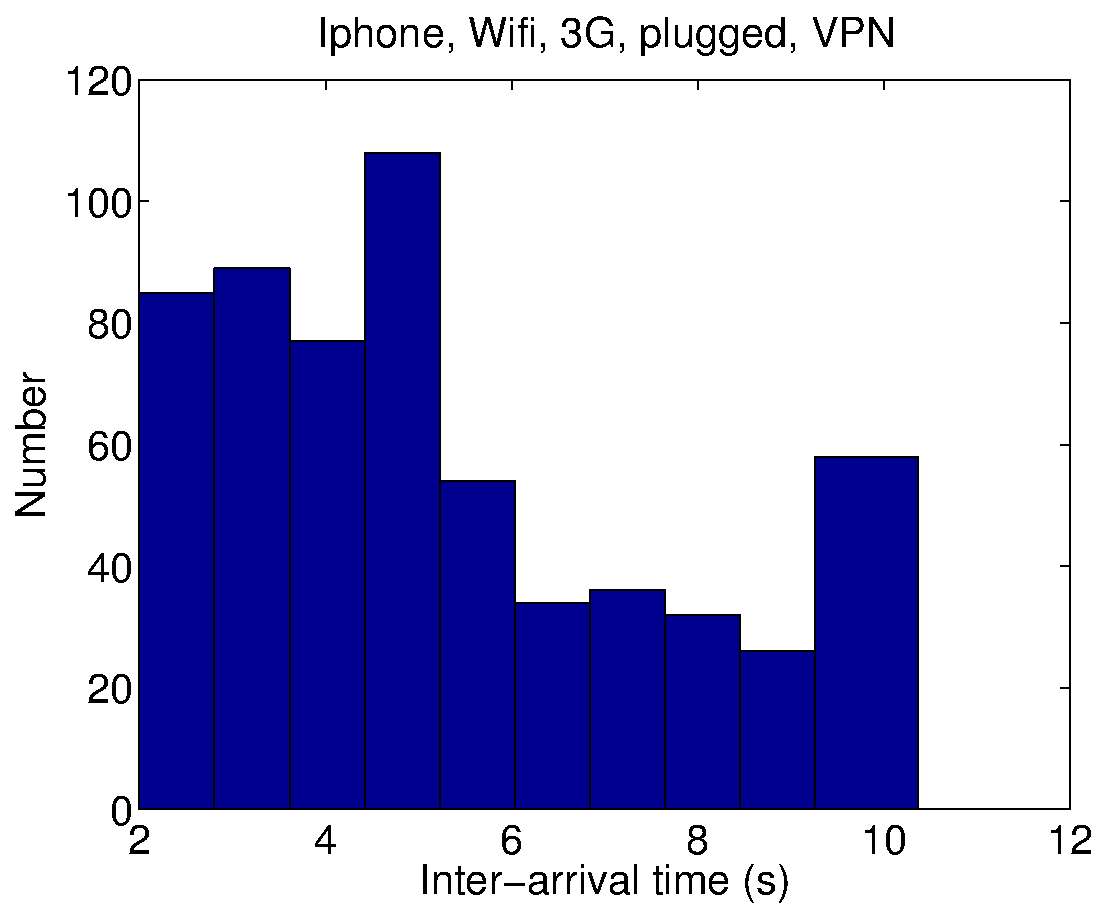
\includegraphics[width=0.8\linewidth]{../../code/pushNotification/Fig/bw_iphone_wifi_3g_plug_vpn_interTs.pdf}
  \caption{Distribution of the interarrival times of Ethernet frames
    for a one hour experiment with an idle \iphone{} plugged-in, with \wifi{} and 3G
    enabled, and VPN enabled. For each bin of 1 second, we count
    the number of interarrivals in that bin.}
  \label{fig:push_w3pv_interTs}
\end{figure}

\begin{figure}
\centering
        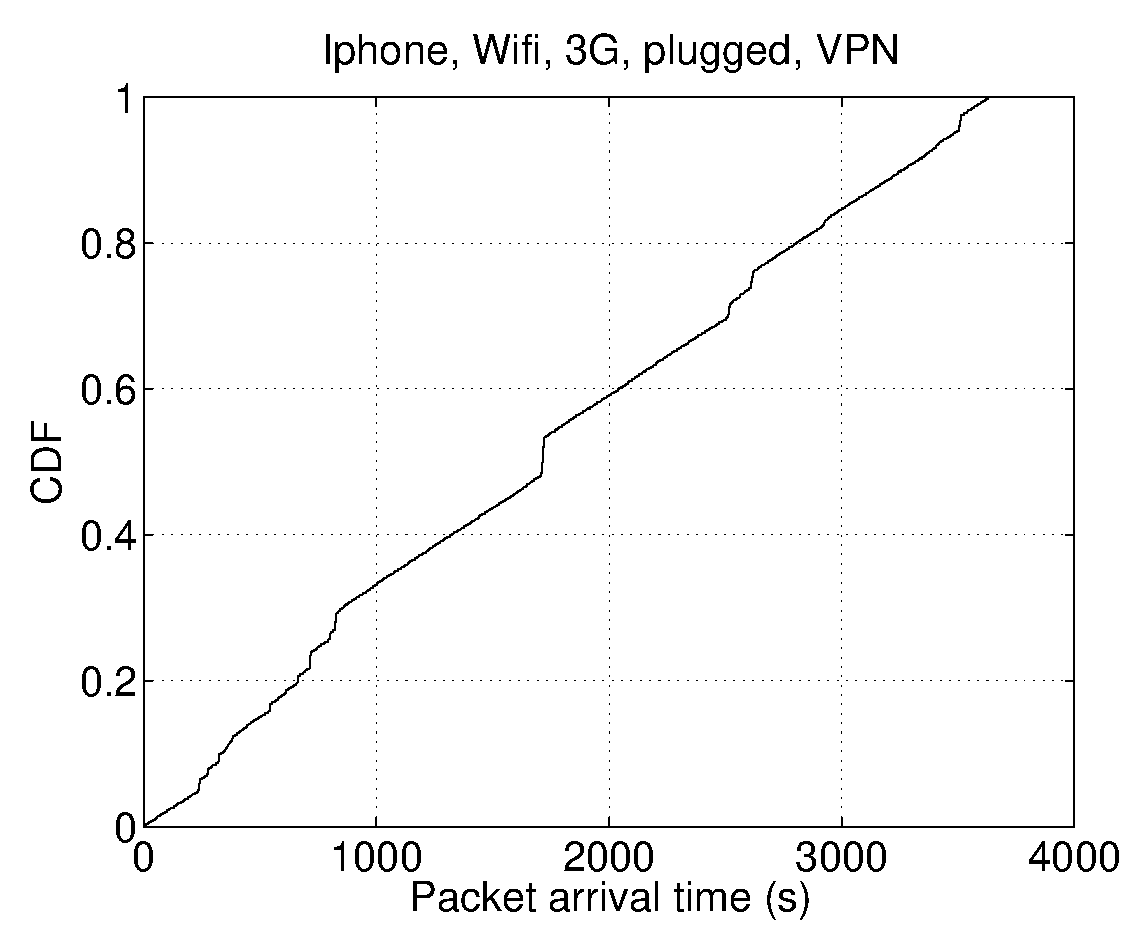
\includegraphics[width=0.8\linewidth]{../../code/pushNotification/Fig/bw_iphone_wifi_3g_plug_vpn_ts.eps}
  \caption{Cumulative distribution of the Ethernet frames
          arrival with time for a one hour experiment with an idle
          \iphone{} plugged-in, with \wifi{} and 3G enabled, and VPN
          enabled.}
  \label{fig:push_w3pv_ts}
\end{figure}

When an \iphone{} is plugged-in, it always remains associated to the
\wifi{} access point if \wifi{} is enabled on the device. We performed
a first set of experiments to observe the traffic to and from an idle
\iphone{}. We see in Fig.~\ref{fig:push_w3p_interTs} and
Fig.~\ref{fig:push_w3pv_interTs} that the largest interarrival between
two frames is in the order of 10 seconds for both the VPN and no VPN
scenarios. We also observe no noticeable difference in the arrival of
frames with time for both the VPN (see Fig.~\ref{fig:push_w3pv_ts} and
no VPN (see Fig.~\ref{fig:push_w3p_ts}) scenarios. We don't claim this
traffic to be typical, in particular, our access point is a Windows 7
machine sending SSDP traffic to announce available services. Instead,
we use it to understand in our experimental setup the background
traffic.





\begin{figure}
\centering
        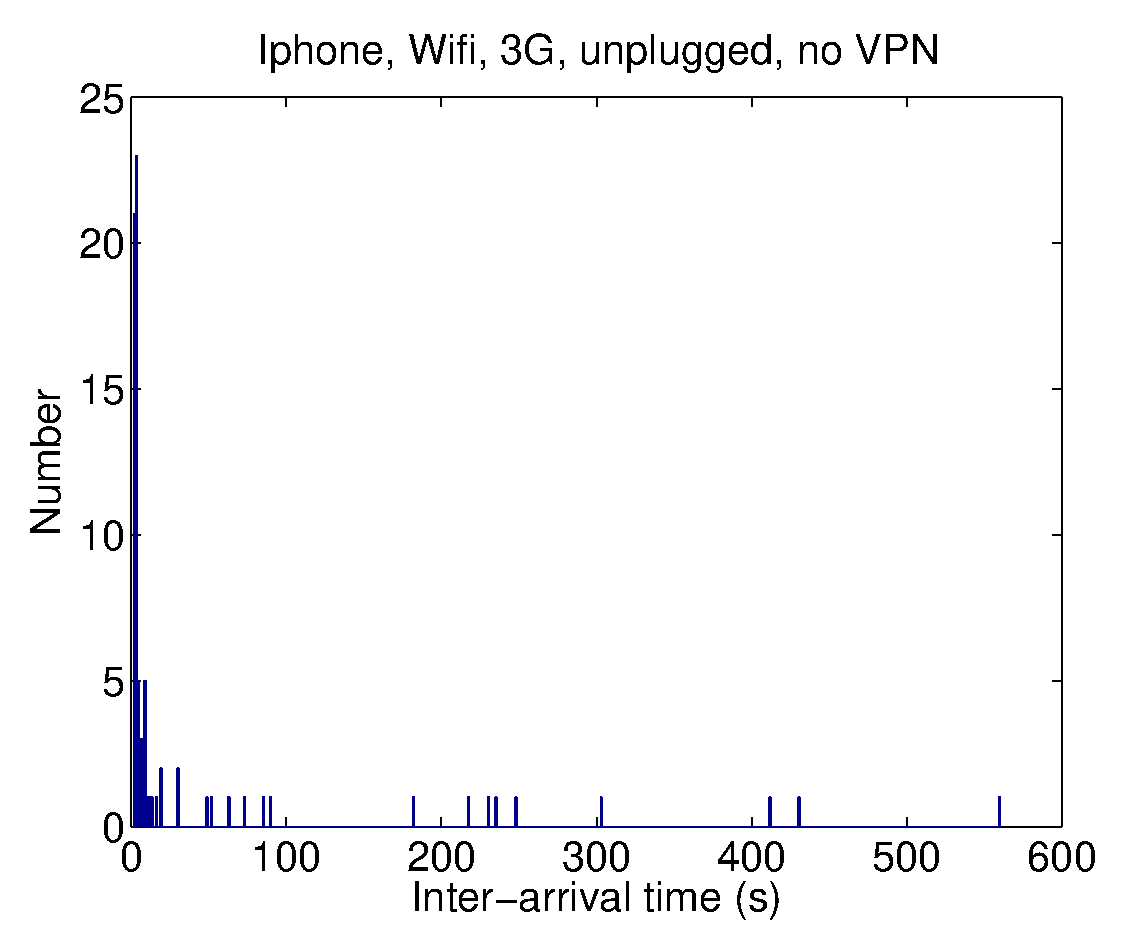
\includegraphics[width=0.8\linewidth]{../../code/pushNotification/Fig/bw_iphone_wifi_3g_unplug_novpn_interTs.eps}
  \caption{Distribution of the interarrival times of Ethernet frames
    for a one hour experiment with an idle \iphone{} unplugged, with \wifi{} and 3G
    enabled, and no VPN enabled. For each bin of 1 second, we count
    the number of interarrivals in that bin.}
  \label{fig:push_w3_interTs}
\end{figure}

\begin{figure}
\centering
        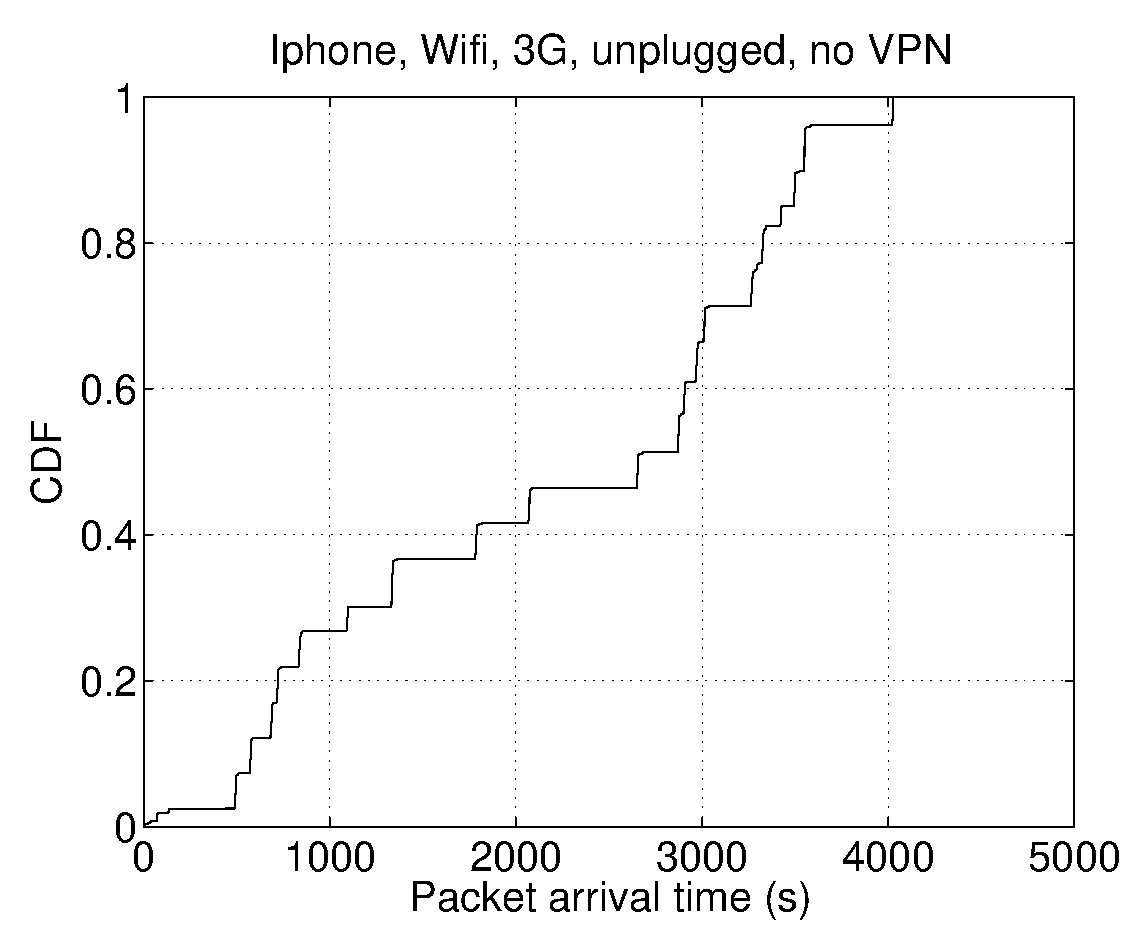
\includegraphics[width=0.8\linewidth]{../../code/pushNotification/Fig/bw_iphone_wifi_3g_unplug_novpn_ts.eps}
  \caption{Cumulative distribution of the Ethernet frames
          arrival with time for a one hour experiment with an idle
          \iphone{} unplugged, with \wifi{} and 3G enabled, and no VPN
          enabled.}
  \label{fig:push_w3_ts}
\end{figure}

In a second set of experiments, we consider a default \iphone{}
setting with 3G and \wifi{} enabled, and the \iphone{} unplugged. This
corresponds to a typical setting for a user on move.  We observe in
Fig.~\ref{fig:push_w3_interTs} some very large frames interarrival
times. All interarrival times larger than 10 seconds correspond to
periods during which the wifi interface of the \iphone{} is not
associated to the access point for energy saving. Surprisingly,
whereas the \iphone{} is idle, we do not observe any regular pattern
in the arrival of the frames in Fig.~\ref{fig:push_w3_ts}. In order to
understand this irregularity, we made a new experiment with 3G
disabled.


\begin{figure}
\centering
        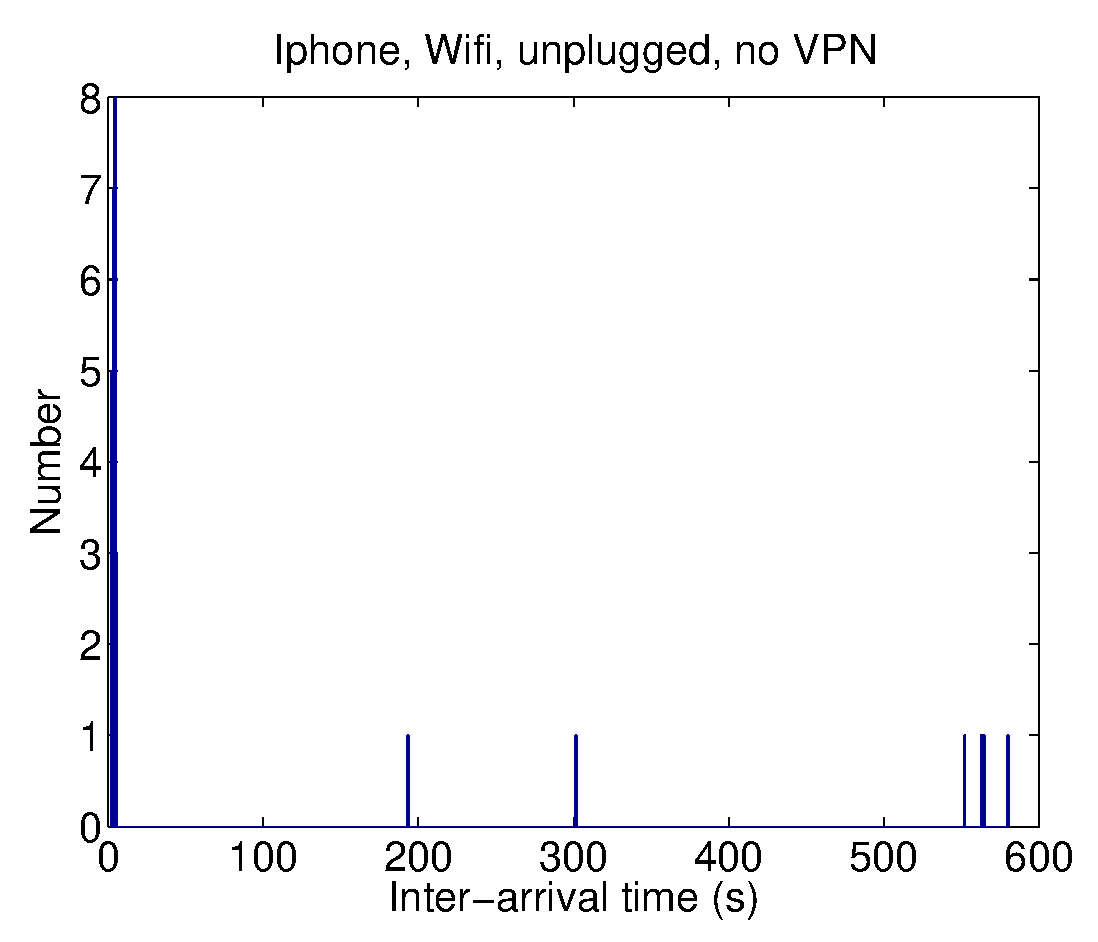
\includegraphics[width=0.8\linewidth]{../../code/pushNotification/Fig/bw_iphone_wifi_unplug_novpn_interTs.eps}
  \caption{Distribution of the interarrival times of Ethernet frames
    for a one hour experiment with an idle \iphone{} unplugged, with \wifi{} 
    enabled, and no VPN enabled. For each bin of 1 second, we count
    the number of interarrivals in that bin.}
  \label{fig:push_w_interTs}
\end{figure}

\begin{figure}
\centering
        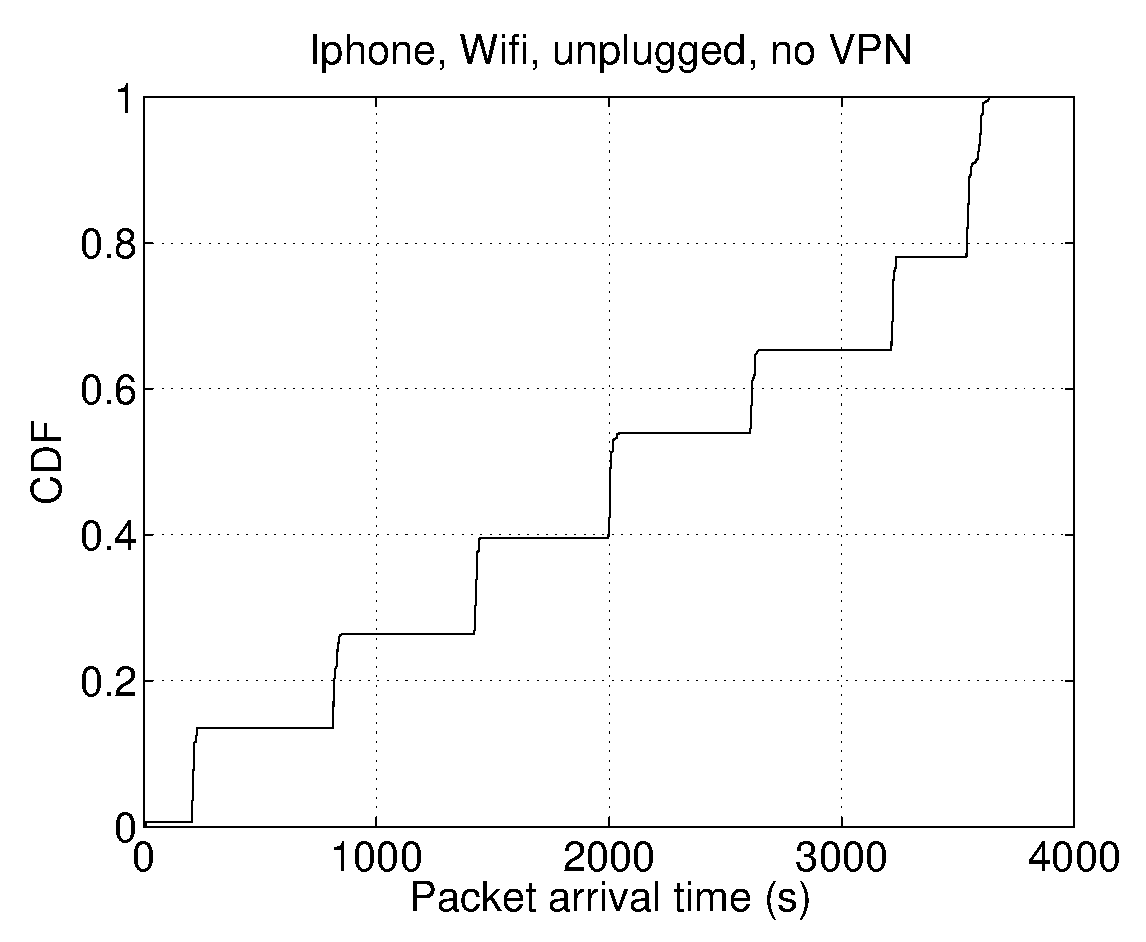
\includegraphics[width=0.8\linewidth]{../../code/pushNotification/Fig/bw_iphone_wifi_unplug_novpn_ts.eps}
  \caption{Cumulative distribution of the Ethernet frames
          arrival with time for a one hour experiment with an idle
          \iphone{} unplugged, with \wifi{} enabled, and no VPN
          enabled.}
  \label{fig:push_w_ts}
\end{figure}

We observe in Fig.~\ref{fig:push_w_interTs} that the largest
interarrival is still in the order of 550 seconds, as in the case with
3G enabled, but we have less variety in the interarrival times. This
is confirmed by Fig.~\ref{fig:push_w_ts} that shows a regular
succession of short periods during which frames are received and long
periods during which the wifi connection is not associated to the
access point.

Therefore, there is an evidence that the 3G connection might trigger
the association of the \iphone{} wifi interface with the access
point. This is confirmed by experiments we performed with iMessage
that is using the push notification infrastructure of Apple. When both
3G and \wifi{} are enabled on an \iphone{}, a permanent connection to
the push notification infrastructure of Apple is setup on the 3G
interface. Each time an iMessage is received, it is piggybacked on the
push notification message (when short enough). However, the \wifi{}
interface is always woken-up even if no payload is sent on it. 

We observed this same behavior on the tcpdump traces used to plot
Fig.~\ref{fig:push_w3_ts}. We observe that the \wifi{} interface is
woken-up (we observe a specific ARP and DHCP exchange that takes place
for each \wifi{} association to the access point), but no payload is
exchanged. In this case, as we do not use a VPN, we cannot monitor the
3G traffic using \meddle{}, but we guess that traffic received on the
3G interface trigger the wake of the \wifi{} interface. We plan to
further explore this issue. 


\begin{figure}
\centering
        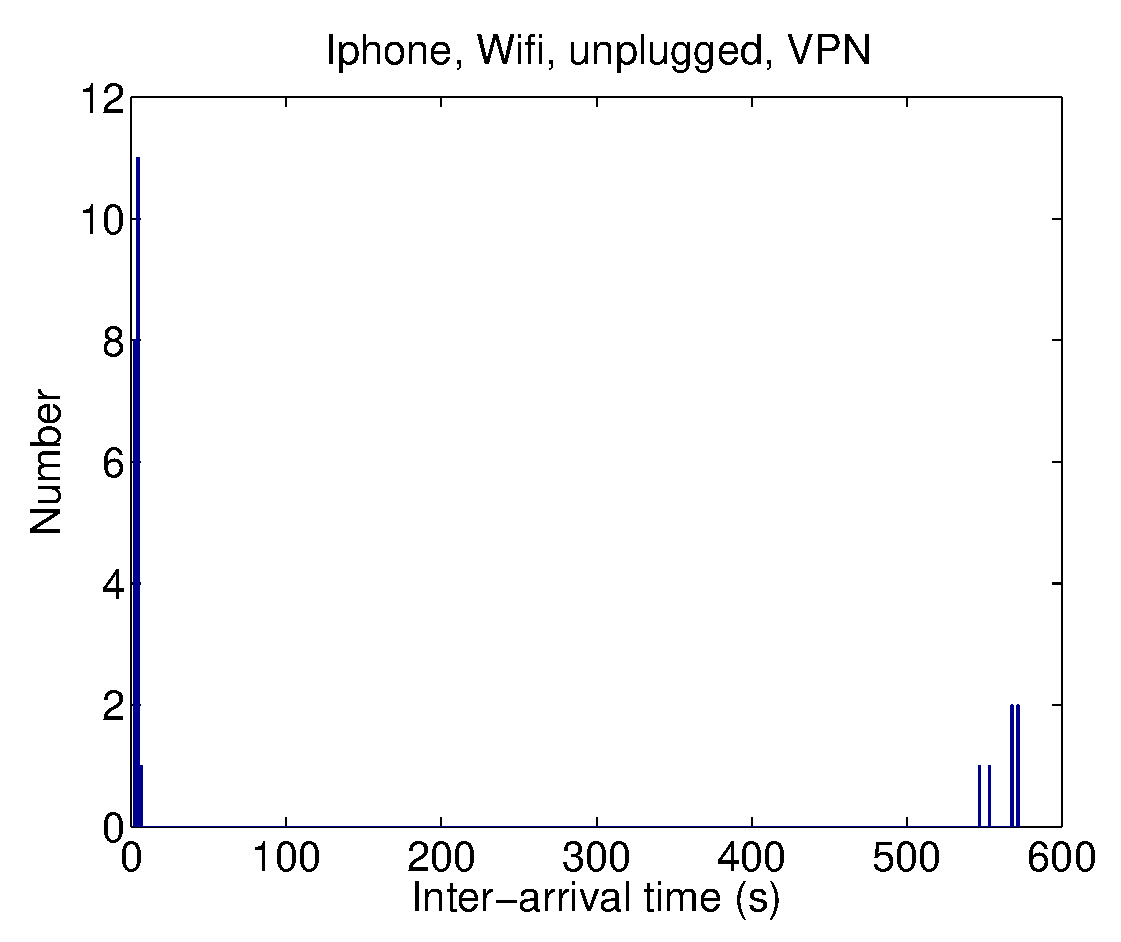
\includegraphics[width=0.8\linewidth]{../../code/pushNotification/Fig/bw_iphone_wifi_unplug_vpn_interTs.eps}
  \caption{Distribution of the interarrival times of Ethernet frames
    for a one hour experiment with an idle \iphone{} unplugged, with \wifi{}
    enabled, and VPN enabled. For each bin of 1 second, we count
    the number of interarrivals in that bin.}
  \label{fig:push_wv_interTs}
\end{figure}

\begin{figure}
\centering
        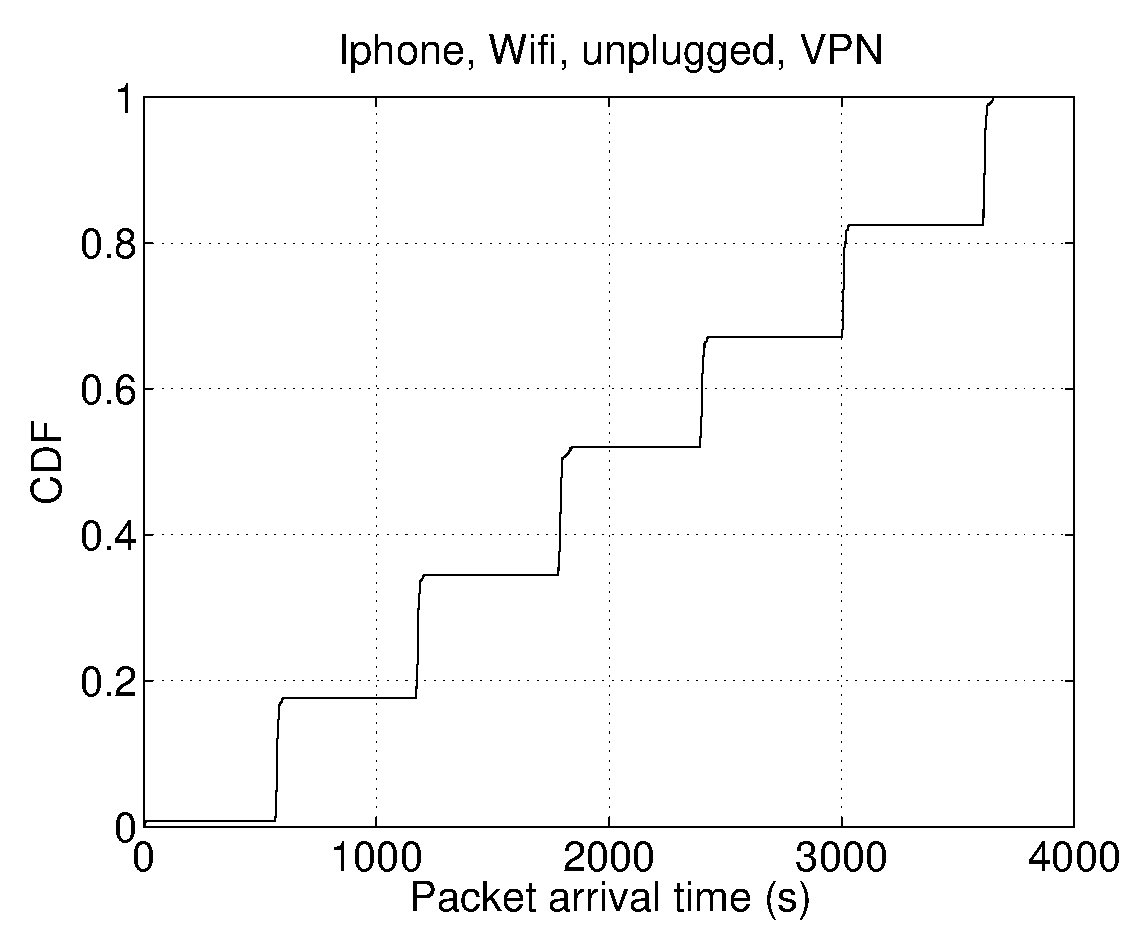
\includegraphics[width=0.8\linewidth]{../../code/pushNotification/Fig/bw_iphone_wifi_unplug_vpn_ts.eps}
  \caption{Cumulative distribution of the Ethernet frames
          arrival with time for a one hour experiment with an idle
          \iphone{} unplugged, with \wifi{} enabled, and VPN
          enabled.}
  \label{fig:push_wv_ts}
\end{figure}

We performed a third set of experiments with the VPN enabled. This set
of experiment shows the impact of using \meddle on the traffic pattern
and the power management policy. We see in
Fig.~\ref{fig:push_wv_interTs} and Fig.~\ref{fig:push_wv_ts} that
there is no noticeable differences when enabling \meddle with \wifi{} only. However,
when enabling both \wifi and 3G the frames interarrival time
(Fig.~\ref{fig:push_w3v_interTs}) and the cumulative arrival of frames
(Fig.~\ref{fig:push_w3v_ts}) is significantly different. 
\tbd{It will probably be too short for the deadline, but I need to see
on the meddle logs what are these 3G messages. I cannot get them from
my setup. I guess that the VPN is using keep alive message every 45
seconds. As the 3G connection never sleep, receiving such a packet
trigger the wake-up of the \wifi{} interface. When 3G is disabled, the
keep alive messages cannot prevent the \wifi{} interface to
sleep. Ashwin, if you are aware of such a timer in your VPN config, we
can safely state my guess in the paper.}





\begin{figure}
\centering
        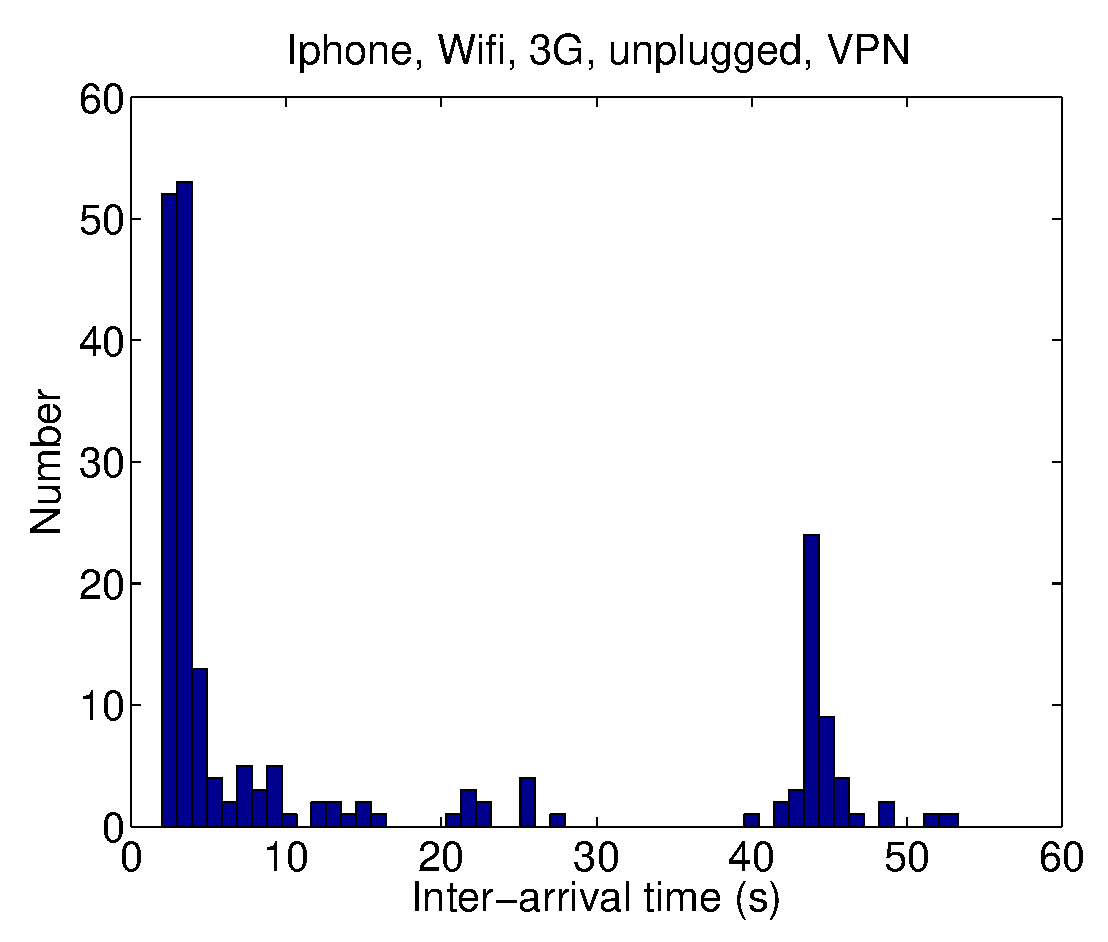
\includegraphics[width=0.8\linewidth]{../../code/pushNotification/Fig/bw_iphone_wifi_3g_unplug_vpn_interTs.eps}
  \caption{Distribution of the interarrival times of Ethernet frames
    for a one hour experiment with an idle \iphone{} unplugged, with \wifi{} and 3G
    enabled, and VPN enabled. For each bin of 1 second, we count
    the number of interarrivals in that bin.}
  \label{fig:push_w3v_interTs}
\end{figure}

\begin{figure}
\centering
        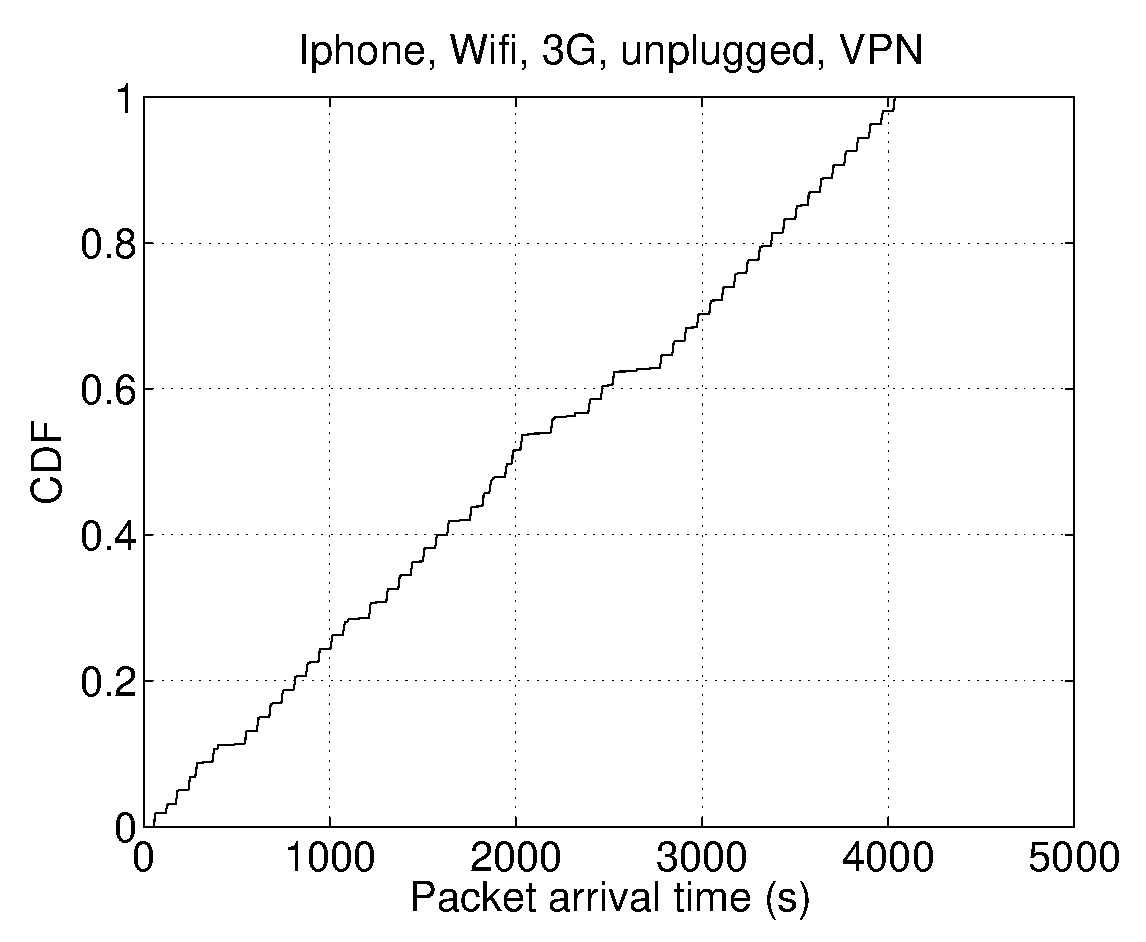
\includegraphics[width=0.8\linewidth]{../../code/pushNotification/Fig/bw_iphone_wifi_3g_unplug_vpn_ts.eps}
  \caption{Cumulative distribution of the Ethernet frames
          arrival with time for a one hour experiment with an idle
          \iphone{} unplugged, with \wifi{} and 3G enabled, and VPN
          enabled.}
  \label{fig:push_w3v_ts}
\end{figure}


%%% Local Variables: 
%%% mode: latex
%%% TeX-master: "main"
%%% End: 
